\section{Banco de dados relacional}

\begin{frame}
	\begin{block}{Banco de dados relacional}
		\begin{itemize}
			\item Antes de computadores a informação era armazenada em papel. Isso tornava o processo de análise, armazenamento e leitura de informação trabalhoso e demorado (Ficheiros são uma forma de indexação).
			
			\item Nos anos 60 surgiram os sistemas de arquivo (precisávamos conhecer as estruturas dos arquivos para pesquisar)
			
			\item Nos anos 70 surgiram os Sistemas Gerenciadores de Banco de Dados (SGBD) com o modelo de dados relacional
			
			\item Nos anos 80 o uso de banco de dados é difundido em meio acadêmico, surge o SQL.
			
			\item Anos 90, grandes empresas fornecedoras de SGBD, Microsoft,. Oracle, IBM, ... E software livre como MySql, Firebird, Postgresql
		\end{itemize}
	\end{block}
\end{frame}

\begin{frame}
	\begin{block}{SQL}
		\begin{itemize}
			\item Structured Query Language (SQL) linguagem para consulta de banco de dados relacionais padronizada entre diferentes bancos de dados. 

			\item Vale ressaltar que nem todo banco de dados segue apenas o padrão SQL, cada distribuidor de ferramenta implementa algumas funcionalidades extras para facilitar o trabalho do DBA.
		\end{itemize}
	\end{block}
\end{frame}

\begin{frame}
	\begin{block}{Banco de dados relacional}
		\begin{itemize}
			\item Atualmente SGBD podem ser executados em simples computadores pessoais. 
			
			\item Algumas definições:
			
			\item Dado: representação da informação: classe do herói, cor da roupa, 
			      tipo de arma
			
			\item Informação: Fato extraído de um conjunto de dados e.g. Guerreiro com nível de experiência 98, peso 105 Kg morador de Gondor pertencente a cavalaria real.
		\end{itemize}
	\end{block}
\end{frame}

\begin{frame}
	\begin{block}{Banco de dados relacional}
		\begin{itemize}
			\item Conjunto de tabelas relacionadas armazenadas em disco rígido (HD) em uma estrutura de dados eficiente para leitura e escrita.
			
			\item Garantem consistência dos dados, atomicidade de operações, isolamento, durabilidade (ACID)
				
			\item Permitem que se construa uma estrutura que evita redundância de informação, se corretamente normalizado.
		\end{itemize}
	\end{block}
\end{frame}


\begin{frame}
	\begin{block}{Comandos SQL}
		\begin{itemize}
			\item Vamos estudar os comandos para manipular dados em bancos de dados relacionais (select, create, update, delete, ...). 

			\item Comandos de gerenciamento e definição de dados não serão avaliados (grant, revoke, index, ....)
			
			\item Vamos usar um banco de dados de exemplo em SQLite um banco de dados que não exige SGBD, tipicamente usado em dispositivos móveis (como celulares)
		\end{itemize}
	\end{block}
\end{frame}

\begin{frame}
	\begin{table}[]
		\begin{tabular}{|l|l|}
		\hline
			\textbf{Comando} & \textbf{Descrição}                      \\ \hline
			SELECT           & Seleciona colunas da tabela             \\ \hline
			INSERT           & Insere registros na tabela              \\ \hline
			UPDATE           & Atualiza valores das colunas da tabela  \\ \hline
			DELETE           & Deleta linhas da tabela                 \\ \hline
			CREATE           & Cria tabelas                            \\ \hline
			ALTER            & Altera estrutura das tabelas            \\ \hline
			DROP             & Deleta tabelas e outros objetos do SGBD \\ \hline
			HAVING           & Filtra linhas agrupadas                 \\ \hline
			GROUP BY         & Agrupa dados                            \\ \hline
			WHERE            & Filtra linhas não agrupadas             \\ \hline
		\end{tabular}
	\end{table}
\end{frame}

%#https://www.devmedia.com.br/sql-join-entenda-como-funciona-o-retorno-dos-dados/31006
\begin{frame}
	\begin{block}{JOINS SQL}
		\begin{figure}[!htb]
			\centering	  				
			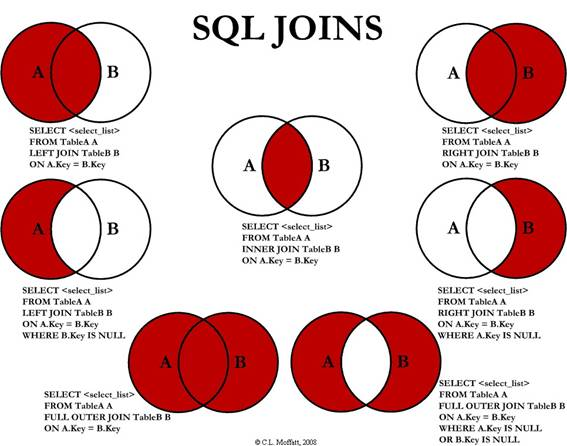
\includegraphics[height=7cm, width = 11cm]{./pic/sqlJoins.jpg}
			\caption{Joins do SQL}
			\label{fig_Joins_sql}
		\end{figure}
	\end{block}
\end{frame}

%http://www.sqlitetutorial.net/sqlite-sample-database/
\begin{frame}
	\begin{block}{Base de Exemplo}
		\begin{figure}[!htb]
			\centering	  				
			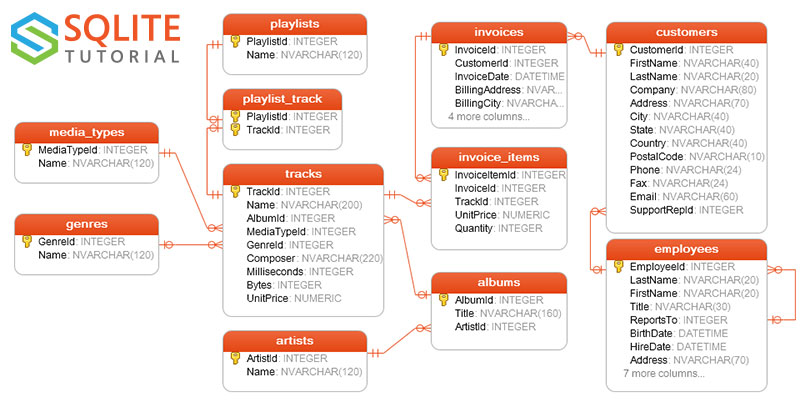
\includegraphics[height=7cm, width = 11cm]{./pic/sqlite-sample-database-color.jpg}
			\caption{Base de Exemplo}
			\label{fig_Joins_sql}
		\end{figure}
	\end{block}
\end{frame}

\begin{frame}[fragile]
	\begin{block}{Select}	
	Comando para selecionar determinadas colunas de uma (ou mais) tabelas do banco de dados:
				\inputminted[linenos,
									fontsize=\footnotesize,
									baselinestretch=1.2,
									framesep=2mm,
									bgcolor=bg_gray, 
									frame=lines]
									{sql}
									{./secoes/BancoDeDados/select.sql}
	\end{block}
\end{frame}

\begin{frame}[fragile]
	\begin{block}{Select asterísco}	
		Comando para selecionar todas as colunas de uma (ou mais) tabelas do banco de dados:
				\inputminted[linenos,
									fontsize=\footnotesize,
									baselinestretch=1.2,
									framesep=2mm,
									bgcolor=bg_gray, 
									frame=lines]
									{sql}
									{./secoes/BancoDeDados/selectasterisco.sql}
	\end{block}
\end{frame}

\begin{frame}[fragile]
	\begin{block}{Order by ASC}	
	Comando para ordernar os registros (maior para o menor) de acordo com a coluna seguinte ao comando:
				\inputminted[linenos,
									fontsize=\footnotesize,
									baselinestretch=1.2,
									framesep=2mm,
									bgcolor=bg_gray, 
									frame=lines]
									{sql}
									{./secoes/BancoDeDados/orderby.sql}
	\end{block}
\end{frame}

\begin{frame}[fragile]
	\begin{block}{Order by DESC} 	
	Comando para ordernar os registros (menor para o maior) de acordo com a coluna seguinte ao comando:
				\inputminted[linenos,
									fontsize=\footnotesize,
									baselinestretch=1.2,
									framesep=2mm,
									bgcolor=bg_gray, 
									frame=lines]
									{sql}
									{./secoes/BancoDeDados/orderbydesc.sql}
	\end{block}
\end{frame}

\begin{frame}[fragile]
	\begin{block}{Where} 	
	Comando para filtrar linhas:
				\inputminted[linenos,
									fontsize=\footnotesize,
									baselinestretch=1.2,
									framesep=2mm,
									bgcolor=bg_gray, 
									frame=lines]
									{sql}
									{./secoes/BancoDeDados/where.sql}
	\end{block}
\end{frame}

\begin{frame}[fragile]
	\begin{block}{Like} 	
	Comando de expressão regular para filtrar linhas:
				\inputminted[linenos,
									fontsize=\footnotesize,
									baselinestretch=1.2,
									framesep=2mm,
									bgcolor=bg_gray, 
									frame=lines]
									{sql}
									{./secoes/BancoDeDados/coringa.sql}
	\end{block}
\end{frame}

\begin{frame}[fragile]
	\begin{block}{In} 	
	Comando para determinar range de valores finitos, tipicamente usado em condições case ou where:
				\inputminted[linenos,
									fontsize=\footnotesize,
									baselinestretch=1.2,
									framesep=2mm,
									bgcolor=bg_gray, 
									frame=lines]
									{sql}
									{./secoes/BancoDeDados/in.sql}
	\end{block}
\end{frame}

\begin{frame}[fragile]
	\begin{block}{Inner Join} 	
	Comando para juntar tabelas, apenas registros que existem em ambas as tabelas:
				\inputminted[linenos,
									fontsize=\footnotesize,
									baselinestretch=1.2,
									framesep=2mm,
									bgcolor=bg_gray, 
									frame=lines]
									{sql}
									{./secoes/BancoDeDados/innerjoin.sql}
	\end{block}
\end{frame}

\begin{frame}[fragile]
	\begin{block}{Left Join} 	
		Comando para juntar tabelas, apenas registros que existem em ambas as tabelas ou na tabela da esquerda:
				\inputminted[linenos,
									fontsize=\footnotesize,
									baselinestretch=1.2,
									framesep=2mm,
									bgcolor=bg_gray, 
									frame=lines]
									{sql}
									{./secoes/BancoDeDados/leftjoin.sql}
	\end{block}
\end{frame}


\begin{frame}[fragile]
	\begin{block}{Count} 	
	Comando de agregação para sumarizar dados, nesse caso contá-los:
				\inputminted[linenos,
									fontsize=\footnotesize,
									baselinestretch=1.2,
									framesep=2mm,
									bgcolor=bg_gray, 
									frame=lines]
									{sql}
									{./secoes/BancoDeDados/count.sql}
	\end{block}
\end{frame}

\begin{frame}[fragile]
	\begin{block}{Union} 	
	Comando para juntar dois selects empilhando as colunas de ambos:
				\inputminted[linenos,
									fontsize=\footnotesize,
									baselinestretch=1.2,
									framesep=2mm,
									bgcolor=bg_gray, 
									frame=lines]
									{sql}
									{./secoes/BancoDeDados/union.sql}
	\end{block}
\end{frame}

\begin{frame}[fragile]
	\begin{block}{Having} 	
	Comando para filtrar resultados agrupados:
				\inputminted[linenos,
									fontsize=\footnotesize,
									baselinestretch=1.2,
									framesep=2mm,
									bgcolor=bg_gray, 
									frame=lines]
									{sql}
									{./secoes/BancoDeDados/having.sql}
	\end{block}
\end{frame}

\begin{frame}[fragile]
	\begin{block}{Insert} 	
	Comando para inserir registros no banco de dados:
				\inputminted[linenos,
									fontsize=\footnotesize,
									baselinestretch=1.2,
									framesep=2mm,
									bgcolor=bg_gray, 
									frame=lines]
									{sql}
									{./secoes/BancoDeDados/insert.sql}
	\end{block}
\end{frame}

\begin{frame}[fragile]
	\begin{block}{Update} 	
	Comando para atualizar registros do banco de dados:
				\inputminted[linenos,
									fontsize=\footnotesize,
									baselinestretch=1.2,
									framesep=2mm,
									bgcolor=bg_gray, 
									frame=lines]
									{sql}
									{./secoes/BancoDeDados/update.sql}
	O que ocorre se esquecermos a cláusula where?
	\end{block}
\end{frame}

\begin{frame}[fragile]
	\begin{block}{Delete} 	
		Comando para deletar registros do banco de dados:
				\inputminted[linenos,
									fontsize=\footnotesize,
									baselinestretch=1.2,
									framesep=2mm,
									bgcolor=bg_gray, 
									frame=lines]
									{sql}
									{./secoes/BancoDeDados/delete.sql}
		O que ocorre se esquecermos a cláusula where?
	\end{block}
\end{frame}


\begin{frame}[fragile]
	\begin{block}{Case} 	
	Comando para tomar decisões sobre valores, seria o equivalente ao if:
				\inputminted[linenos,
									fontsize=\footnotesize,
									baselinestretch=1.2,
									framesep=2mm,
									bgcolor=bg_gray, 
									frame=lines]
									{sql}
									{./secoes/BancoDeDados/case.sql}
	\end{block}
\end{frame}

\begin{frame}[fragile]
	\begin{block}{Alter} 	
		Comando para alterar objetos do banco de dados , entre outros, nomes de tabelas:
				\inputminted[linenos,
									fontsize=\footnotesize,
									baselinestretch=1.2,
									framesep=2mm,
									bgcolor=bg_gray, 
									frame=lines]
									{sql}
									{./secoes/BancoDeDados/alter.sql}
	\end{block}
\end{frame}

\begin{frame}
	\begin{block}{Exercícios}
			\begin{itemize}
				\item Acessar o site \href{http://www.sqlitetutorial.net/}{\color{blue}{SqliteTutorial}} e realizar os tutorias:
				\item Select
				\item Order by
				\item Where
				\item IN
				\item Like
				\item Todos os joins!
				\item Union
				\item Having 
				\item Case
				\item Insert, Update, Delete
				\item Group by e SQLITE functions (AVG, MIN, MAX, SUM)	
			\end{itemize}
	\end{block}
\end{frame}
